% =============================================================================
%  Hera Datasheet
%  Paged KV Cache Memory Controller — Circle Layer 0 IP
%  Version 1.0 | June 2026
%
%  Build:  pdflatex hera_datasheet.tex   (run twice for cross-references)
%  Requires: TeX Live 2022+ or MiKTeX 22+
% =============================================================================

\documentclass[10pt, a4paper]{article}

% ── Encoding & font ───────────────────────────────────────────────────────────
\usepackage[T1]{fontenc}
\usepackage[utf8]{inputenc}
\usepackage[scaled=0.92]{helvet}
\renewcommand{\familydefault}{\sfdefault}
\usepackage{microtype}

% ── Page geometry ─────────────────────────────────────────────────────────────
\usepackage[
  a4paper,
  top=22mm, bottom=26mm,
  left=20mm, right=20mm,
  headheight=15pt
]{geometry}

% ── Colours ───────────────────────────────────────────────────────────────────
\usepackage[table, dvipsnames]{xcolor}
\definecolor{heradark}{HTML}{1A1730}
\definecolor{heraviolet}{HTML}{5B4FCF}
\definecolor{heralight}{HTML}{EEEAF8}
\definecolor{herarule}{HTML}{C5BBEE}
\definecolor{tabhead}{HTML}{F3F1FB}
\definecolor{tabalt}{HTML}{FAFAFA}
\definecolor{codebg}{HTML}{F5F4F9}
\definecolor{muted}{HTML}{555566}
\definecolor{noteframe}{HTML}{DDD8F5}

% ── Graphics & TikZ ───────────────────────────────────────────────────────────
\usepackage{graphicx}
\usepackage{tikz}
\usetikzlibrary{shapes.geometric, arrows.meta, positioning, fit,
                backgrounds, calc, decorations.pathreplacing}

% ── Tables ────────────────────────────────────────────────────────────────────
\usepackage{booktabs}
\usepackage{array}
\usepackage{multirow}
\usepackage{multicol}
\usepackage{tabularx}
\usepackage{longtable}

% ── Headers & footers ─────────────────────────────────────────────────────────
\usepackage{fancyhdr}
\pagestyle{fancy}
\fancyhf{}
\renewcommand{\headrulewidth}{0pt}
\fancyhead[L]{%
  \begin{tikzpicture}[remember picture, overlay]
    \draw[herarule, line width=0.5pt]
      ([yshift=-2pt]current page.north west) ++(\dimexpr\oddsidemargin+1in, -\dimexpr\topmargin+1in+\headheight)
      -- +(\textwidth, 0);
  \end{tikzpicture}%
  \small\color{muted}\textbf{Hera} \textemdash{} Paged KV Cache Memory Controller%
}
\fancyhead[R]{\small\color{muted}Version 1.0 \textbar{} June 2026}
\fancyfoot[C]{\small\color{muted}\thepage}
\fancyfoot[R]{\small\color{muted}\copyright{} 2026 Circle. Apache~License~2.0.}

% ── Section formatting ────────────────────────────────────────────────────────
\usepackage{titlesec}
\titleformat{\section}
  {\large\bfseries\color{heradark}}
  {\color{heraviolet}\thesection}{0.8em}{}[{\color{herarule}\vspace{2pt}\hrule height 0.8pt}]
\titleformat{\subsection}
  {\normalsize\bfseries\color{heradark}}
  {\thesubsection}{0.8em}{}
\titleformat{\subsubsection}
  {\small\bfseries\color{heradark}}
  {\thesubsubsection}{0.8em}{}
\titlespacing{\section}{0pt}{16pt}{6pt}
\titlespacing{\subsection}{0pt}{10pt}{4pt}
\titlespacing{\subsubsection}{0pt}{8pt}{3pt}

% ── Lists ─────────────────────────────────────────────────────────────────────
\usepackage{enumitem}
\setlist{noitemsep, topsep=3pt, leftmargin=1.4em}
\setlist[itemize]{label={\color{heraviolet}\textbullet}}

% ── Paragraph spacing ─────────────────────────────────────────────────────────
\usepackage{parskip}
\setlength{\parskip}{5pt}
\setlength{\parindent}{0pt}

% ── Hyperlinks ────────────────────────────────────────────────────────────────
\usepackage{hyperref}
\hypersetup{
  colorlinks = true,
  linkcolor  = heraviolet,
  urlcolor   = heraviolet,
  citecolor  = heraviolet,
  pdftitle   = {Hera — Paged KV Cache Memory Controller Datasheet},
  pdfauthor  = {Circle},
  pdfsubject = {RTL IP Datasheet},
}

% ── Custom column types ───────────────────────────────────────────────────────
\newcolumntype{L}[1]{>{\raggedright\arraybackslash}p{#1}}
\newcolumntype{C}[1]{>{\centering\arraybackslash}p{#1}}
\newcolumntype{R}[1]{>{\raggedleft\arraybackslash}p{#1}}

% ── Utility macros ────────────────────────────────────────────────────────────
\newcommand{\reg}[1]{\texttt{\textbf{#1}}}
\newcommand{\field}[1]{\texttt{#1}}
\newcommand{\hex}[1]{\texttt{0x#1}}
\newcommand{\portname}[1]{\texttt{#1}}
\newcommand{\param}[1]{\texttt{#1}}

% Callout box
\newcommand{\notebox}[2][Note]{%
  \vspace{4pt}
  \noindent
  \setlength{\fboxsep}{7pt}
  \setlength{\fboxrule}{0pt}
  \colorbox{heralight}{%
    \parbox{\dimexpr\linewidth-2\fboxsep}{%
      \small\color{heradark}%
      \textbf{\color{heraviolet}#1\enspace}\ignorespaces#2%
    }%
  }%
  \vspace{4pt}%
}

% ── TikZ styles ───────────────────────────────────────────────────────────────
\tikzset{
  dsbox/.style={
    draw=heraviolet!50, fill=heralight,
    rounded corners=3pt,
    text=heradark, font=\small,
    inner sep=5pt, align=center,
    minimum height=1cm,
  },
  dstopbox/.style={
    draw=heraviolet, fill=white,
    rounded corners=4pt,
    very thick,
    text=heradark,
    inner sep=10pt,
  },
  extbox/.style={
    draw=muted!50, fill=tabalt,
    rounded corners=3pt,
    text=muted, font=\small\itshape,
    inner sep=5pt, align=center,
  },
  sig/.style={->, >=Stealth, heraviolet, semithick},
  siginv/.style={<-, >=Stealth, heraviolet, semithick},
  sigboth/.style={<->, >=Stealth, heraviolet, semithick},
}

% ── Waveform helpers ──────────────────────────────────────────────────────────
\newcommand{\wvH}[3]{% x-start, y, width  (HIGH)
  \draw[heradark, line width=0.9pt] (#1,#2) -- (#1+#3,#2);
}
\newcommand{\wvL}[3]{% x-start, y, width  (LOW)
  \draw[heradark, line width=0.9pt] (#1,#2-0.35) -- (#1+#3,#2-0.35);
}
\newcommand{\wvR}[2]{% x, y  (rising edge)
  \draw[heradark, line width=0.9pt] (#1,#2-0.35) -- (#1,#2);
}
\newcommand{\wvF}[2]{% x, y  (falling edge)
  \draw[heradark, line width=0.9pt] (#1,#2) -- (#1,#2-0.35);
}
\newcommand{\wvBus}[4]{% x-start, y, width, label  (bus / data valid)
  \draw[heradark, line width=0.9pt]
    (#1+0.1, #2)      -- (#1+#3-0.1, #2)
    (#1+0.1, #2-0.35) -- (#1+#3-0.1, #2-0.35)
    (#1,     #2-0.175) -- (#1+0.1, #2)
    (#1,     #2-0.175) -- (#1+0.1, #2-0.35)
    (#1+#3,  #2-0.175) -- (#1+#3-0.1, #2)
    (#1+#3,  #2-0.175) -- (#1+#3-0.1, #2-0.35);
  \node[font=\tiny, heradark] at (#1+#3/2, #2-0.175) {#4};
}

% =============================================================================
\begin{document}
\pagenumbering{arabic}

% =============================================================================
%  COVER PAGE
% =============================================================================
\thispagestyle{empty}

% Top colour bar
\noindent
\begin{tikzpicture}[remember picture, overlay]
  \fill[heradark]
    (current page.north west) rectangle
    ([yshift=-11mm]current page.north east);
\end{tikzpicture}

\vspace*{5mm}

% Top row: classification left, Circle logo right
\noindent
\begin{minipage}[t]{0.55\linewidth}
  \vspace{2pt}
  \small\color{muted} Public Release \textbullet{} Apache License 2.0
\end{minipage}%
\hfill
\begin{minipage}[t]{0.38\linewidth}
  \raggedleft
  
\includegraphics[height=1.05cm]{circle_logo_render}
\end{minipage}

\vspace{22mm}

% Hera wordmark
\noindent
\includegraphics[width=9.5cm]{hera_logo_render}

\vspace{5mm}

\noindent{\LARGE\color{heradark} Paged KV Cache Memory Controller}

\vspace{2mm}

\noindent{\large\color{muted} Synthesizable RTL IP \textbullet{} Circle Layer~0}

\vspace{10mm}
\noindent{\color{herarule}\rule{\linewidth}{0.8pt}}
\vspace{6mm}

% Abstract
\noindent\begin{minipage}{0.90\linewidth}
  \normalsize\color{heradark}
  Hera is a synthesizable RTL IP block that offloads KV cache memory management
  from software to dedicated hardware. It handles page allocation, logical-to-physical
  mapping, scatter-gather reads across non-contiguous pages, sequential prefetch,
  LRU eviction, and multi-tenant isolation — entirely in silicon, with no CPU
  involvement on the critical path. Hera is designed for agentic AI inference
  workloads where multiple concurrent sessions share on-chip SRAM and access
  patterns are irregular across long contexts.
\end{minipage}

\vspace{8mm}

% Quick-spec table
\begin{center}
\small
\setlength{\tabcolsep}{8pt}
\renewcommand{\arraystretch}{1.3}
\begin{tabular}{L{4.4cm} L{3.4cm} L{4.4cm} L{3cm}}
\rowcolor{tabhead}
\multicolumn{2}{l}{\textbf{\color{heradark}Parameter}} &
\multicolumn{2}{l}{\textbf{\color{heradark}Parameter}} \\
\midrule
Total pages            & 256              & Concurrent sessions  & 8 \\
\rowcolor{tabalt}
Page size              & 16 tokens        & Data width           & FP16 (16-bit) \\
Head dimension         & 64               & SRAM footprint       & 1\,MB (default) \\
\rowcolor{tabalt}
Host interface         & AXI4-Lite 32-bit & Target clock         & 100\,MHz \\
Fmax (Artix-7 --1)    & $\approx$126\,MHz & Verification        & 41\,/\,41 checks \\
\rowcolor{tabalt}
Synthesis tool         & Vivado 2018.2    & License              & Apache 2.0 \\
\multicolumn{4}{l}{\small\color{muted}
  Source: \href{https://github.com/anubhavgpta/hera}{github.com/anubhavgpta/hera}} \\
\end{tabular}
\end{center}

\vspace{6mm}

\begin{center}
  \small\color{muted}
  Version 1.0 \textbullet{} June 2026 \textbullet{}
  \href{mailto:anubhavgpta@outlook.com}{anubhavgpta@outlook.com}
\end{center}

\noindent{\color{herarule}\rule{\linewidth}{0.5pt}}

\newpage

% =============================================================================
\section{Features}
% =============================================================================

\begin{multicols}{2}
\begin{itemize}
  \item Paged SRAM management for transformer KV cache — 256 physical pages,
        16 tokens per page, configurable via RTL parameters
  \item One-cycle page allocation and deallocation via circular FIFO free list
        in LUTRAM
  \item Scatter-gather KV read engine with transparent page-boundary crossing
        and valid/ready burst output
  \item AXI4-Lite host interface for runtime configuration, status monitoring,
        and interrupt control
  \item LRU eviction engine with host-acknowledged page scrubbing — 256-cycle
        scan latency
  \item Sequential prefetch: per-session access pattern detector with 2-entry
        prefetch buffer and LRU replacement
  \item Hardware session isolation — cross-session read attempts return zeros
        and latch a security fault
  \item Zero-on-free scrubbing prevents KV data leakage between sessions
  \item Per-session page quota enforcement with IRQ on violation
  \item Sticky LOCK register freezes configuration after boot; survives soft
        reset, cleared only by hard reset
  \item AXI SLVERR on writes to read-only registers, unmapped addresses, and
        locked configuration registers
  \item Silicon watermark: \reg{IP\_VERSION} hardcoded to \hex{48455241}
        (ASCII \texttt{HERA}), recoverable from gate-level netlist
  \item Synthesizes clean at 100\,MHz on Artix-7 xc7a100tcsg324-1, Fmax
        $\approx$126\,MHz
  \item Zero external dependencies — pure Verilog RTL, single-clock design
  \item Apache License 2.0, open source
\end{itemize}
\end{multicols}

% =============================================================================
\section{Architecture}
% =============================================================================

\subsection{System Context}

Hera sits between the host CPU (which configures and monitors via AXI4-Lite)
and the attention engine (which writes and reads KV vectors via dedicated
streaming interfaces). The host allocates sessions, sets quotas, and handles
eviction acknowledgements. The attention engine drives \portname{wr\_req} and
\portname{rd\_req} directly without CPU involvement on the data path.

\subsection{Block Diagram}

\begin{center}
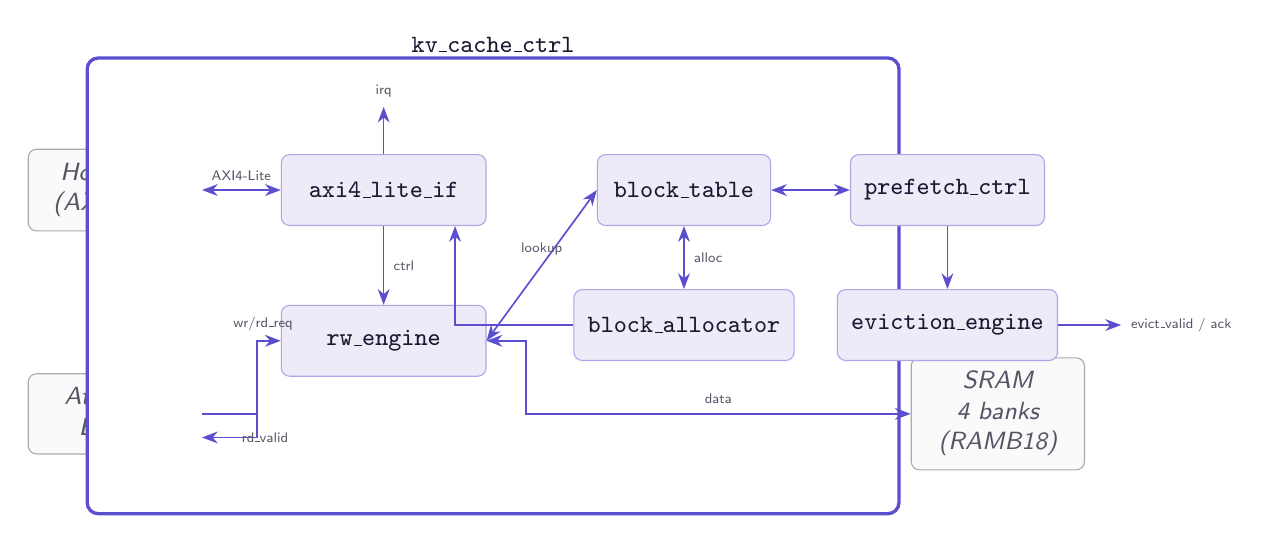
\begin{tikzpicture}[node distance=5mm and 6mm]

  % External actors
  \node[extbox, minimum width=2.2cm] (cpu)
    {Host CPU\\(AXI4-Lite)};
  \node[extbox, minimum width=2.2cm, below=18mm of cpu] (attn)
    {Attention\\Engine};
  \node[extbox, minimum width=2.2cm, right=90mm of attn] (sram)
    {SRAM\\4 banks\\(RAMB18)};

  % Top-level boundary
  \node[dstopbox,
        fit={($(cpu.east)+(5mm,-2mm)$) ($(sram.west)+(-5mm,0)$)
             ($(attn.south)+(0,-4mm)$) ($(cpu.north)+(0,8mm)$)},
        label={[font=\small\bfseries, heradark, yshift=-2pt]north:{\texttt{kv\_cache\_ctrl}}}
       ] (top) {};

  % Internal modules
  \node[dsbox, minimum width=2.6cm, minimum height=0.9cm,
        right=10mm of cpu] (axi)
    {\texttt{axi4\_lite\_if}};

  \node[dsbox, minimum width=2.6cm, minimum height=0.9cm,
        below=10mm of axi] (rwe)
    {\texttt{rw\_engine}};

  \node[dsbox, minimum width=2.2cm, minimum height=0.9cm,
        right=14mm of axi] (bt)
    {\texttt{block\_table}};

  \node[dsbox, minimum width=2.2cm, minimum height=0.9cm,
        below=8mm of bt] (ba)
    {\texttt{block\_allocator}};

  \node[dsbox, minimum width=2.2cm, minimum height=0.9cm,
        right=10mm of bt] (pf)
    {\texttt{prefetch\_ctrl}};

  \node[dsbox, minimum width=2.2cm, minimum height=0.9cm,
        below=8mm of pf] (ev)
    {\texttt{eviction\_engine}};

  % Signals: CPU <-> axi
  \draw[sigboth] (cpu.east) -- (axi.west)
    node[midway, above, font=\tiny, muted] {AXI4-Lite};

  % Signals: axi -> rwe (global_enable / soft_reset)
  \draw[sig] (axi.south) -- (rwe.north)
    node[midway, right, font=\tiny, muted] {ctrl};

  % Signals: attn -> rwe
  \draw[sig] (attn.east) -| ($(rwe.west)+(-3mm,0)$) -- (rwe.west)
    node[near start, above, font=\tiny, muted] {wr/rd\_req};

  % Signals: rwe <-> bt
  \draw[sigboth] (rwe.east) -- (bt.west)
    node[midway, above, font=\tiny, muted] {lookup};

  % Signals: rwe <-> sram
  \draw[sigboth] (rwe.east) -- ++(5mm,0) |- (sram.west)
    node[near end, above, font=\tiny, muted] {data};

  % Signals: bt <-> ba
  \draw[sigboth] (bt.south) -- (ba.north)
    node[midway, right, font=\tiny, muted] {alloc};

  % Signals: ba -> axi (pages_free / status)
  \draw[sig] (ba.west) -| ($(axi.south east)+(-4mm,-5mm)$) -- ++(0,5mm);

  % Signals: ev -> top boundary (evict_valid/ack)
  \draw[sig] (ev.east) -- ++(8mm,0)
    node[right, font=\tiny, muted] {evict\_valid / ack};

  % IRQ
  \draw[sig] (axi.north) -- ++(0,6mm)
    node[above, font=\tiny, muted] {irq};

  % rd_valid back to attn
  \draw[sig] ($(rwe.west)+(-3mm,0)$) |- ($(attn.east)+(0,-3mm)$)
    node[near start, right, font=\tiny, muted] {};
  \node[font=\tiny, muted] at ($(attn.east)+(8mm,-3mm)$) {rd\_valid};

  % pf <-> rwe
  \draw[sig] (pf.south) -- (ev.north)
    node[midway, right, font=\tiny, muted] {};
  \draw[sigboth] (pf.west) -- (bt.east)
    node[midway, above, font=\tiny, muted] {};

\end{tikzpicture}
\end{center}

\subsection{Module Descriptions}

\renewcommand{\arraystretch}{1.35}
\begin{tabularx}{\linewidth}{L{3.2cm} X}
\toprule
\textbf{Module} & \textbf{Description} \\
\midrule
\texttt{block\_allocator}  &
  Maintains a circular FIFO free list in LUTRAM. Provides 1-cycle
  \portname{alloc\_req}/\portname{alloc\_ack} and
  \portname{free\_req}/\portname{free\_ack} handshakes. Outputs
  \portname{pages\_free} (saturates at \hex{FF} when all 256 pages
  are free), \portname{pages\_used}, and \portname{almost\_full}.
  Requires a 256-cycle initialisation pass after any reset. \\
\addlinespace
\texttt{block\_table}  &
  2-D LUTRAM mapping $(\textit{session\_id},\,\textit{logical\_page})
  \rightarrow \textit{physical\_page\_id}$. Single-cycle registered lookup
  with write-first semantics. Supports per-entry invalidation for eviction
  and soft-reset scrubbing. \\
\addlinespace
\texttt{rw\_engine}  &
  Scatter-gather KV read/write engine. Resolves logical token positions
  through the block table and drives the four interleaved SRAM banks.
  Produces a valid/last burst on read. Enforces session ownership on
  every token of a scatter-gather read range. Performs zero-scrub writes
  on behalf of the eviction engine. \\
\addlinespace
\texttt{axi4\_lite\_if}  &
  AXI4-Lite slave. Decodes nine registers (\hex{00}–\hex{24}). Returns
  SLVERR on RO writes, unmapped addresses, and locked configuration
  registers. Latches fault flags and drives the IRQ output. \\
\addlinespace
\texttt{prefetch\_ctrl}  &
  Per-session sequential access detector. On detection of three
  consecutive ascending page accesses, prefetches the next logical page
  into a 2-entry buffer with LRU replacement. \\
\addlinespace
\texttt{eviction\_engine}  &
  Triggered by \portname{almost\_full}. Performs a 256-cycle LRU scan
  over per-page access counters stored in LUTRAM. Presents the LRU
  candidate to the host via \portname{evict\_valid} / \portname{evict\_page\_id}.
  On \portname{evict\_ack}, directs \texttt{rw\_engine} to scrub the
  page to zero before returning it to the free list. \\
\addlinespace
\texttt{kv\_cache\_ctrl}  &
  Top-level integration module. Instantiates all sub-modules, enforces
  RTL parameter guards, sequences zero-on-free scrubbing,
  and arbitrates between normal writes and scrub writes on the
  \texttt{rw\_engine} interface. \\
\bottomrule
\end{tabularx}

% =============================================================================
\section{Signal Descriptions}
% =============================================================================

All ports are synchronous to the rising edge of \portname{clk} unless
otherwise noted. Active-low signals are indicated by the \texttt{\_n} suffix.

\subsubsection*{Clock and Reset}

\renewcommand{\arraystretch}{1.3}
\begin{tabularx}{\linewidth}{L{3cm} C{1.2cm} C{1.4cm} X}
\toprule
\textbf{Signal} & \textbf{Dir} & \textbf{Width} & \textbf{Description} \\
\midrule
\rowcolor{tabalt}
\portname{clk}   & in & 1 & System clock. All registers sample on the rising edge. \\
\portname{rst\_n} & in & 1 & Active-low asynchronous reset. Hold low for $\geq$2 cycles. \\
\bottomrule
\end{tabularx}

\subsubsection*{AXI4-Lite Host Interface (Slave)}

\begin{tabularx}{\linewidth}{L{3.6cm} C{1.2cm} C{1.4cm} X}
\toprule
\textbf{Signal} & \textbf{Dir} & \textbf{Width} & \textbf{Description} \\
\midrule
\rowcolor{tabalt}
\portname{s\_axi\_awvalid} & in  & 1  & Write address valid. \\
\portname{s\_axi\_awready} & out & 1  & Write address ready. \\
\rowcolor{tabalt}
\portname{s\_axi\_awaddr}  & in  & 32 & Write address (byte-addressed; bits [31:8] ignored). \\
\portname{s\_axi\_wvalid}  & in  & 1  & Write data valid. \\
\rowcolor{tabalt}
\portname{s\_axi\_wready}  & out & 1  & Write data ready. \\
\portname{s\_axi\_wdata}   & in  & 32 & Write data. \\
\rowcolor{tabalt}
\portname{s\_axi\_wstrb}   & in  & 4  & Write byte strobes. \\
\portname{s\_axi\_bvalid}  & out & 1  & Write response valid. \\
\rowcolor{tabalt}
\portname{s\_axi\_bready}  & in  & 1  & Write response ready. \\
\portname{s\_axi\_bresp}   & out & 2  & Write response: \hex{00}~=~OKAY, \hex{02}~=~SLVERR. \\
\rowcolor{tabalt}
\portname{s\_axi\_arvalid} & in  & 1  & Read address valid. \\
\portname{s\_axi\_arready} & out & 1  & Read address ready. \\
\rowcolor{tabalt}
\portname{s\_axi\_araddr}  & in  & 32 & Read address. \\
\portname{s\_axi\_rvalid}  & out & 1  & Read data valid. \\
\rowcolor{tabalt}
\portname{s\_axi\_rready}  & in  & 1  & Read data ready. \\
\portname{s\_axi\_rdata}   & out & 32 & Read data. \\
\rowcolor{tabalt}
\portname{s\_axi\_rresp}   & out & 2  & Read response: always OKAY. \\
\portname{irq}             & out & 1  & Level-high interrupt. OR of all unmasked sources. \\
\bottomrule
\end{tabularx}

\subsubsection*{KV Write Interface}

\begin{tabularx}{\linewidth}{L{3.6cm} C{1.2cm} C{1.4cm} X}
\toprule
\textbf{Signal} & \textbf{Dir} & \textbf{Width} & \textbf{Description} \\
\midrule
\rowcolor{tabalt}
\portname{wr\_req}        & in  & 1    & Assert to request a KV write. Hold until \portname{wr\_ack}. \\
\portname{wr\_session\_id}& in  & 3    & Session identifier (0–7). \\
\rowcolor{tabalt}
\portname{wr\_token\_pos} & in  & 12   & Token position within the session's logical address space. \\
\portname{wr\_k\_data}    & in  & 1024 & Key vector ($\text{HEAD\_DIM} \times \text{DATA\_WIDTH}$ bits). \\
\rowcolor{tabalt}
\portname{wr\_v\_data}    & in  & 1024 & Value vector ($\text{HEAD\_DIM} \times \text{DATA\_WIDTH}$ bits). \\
\portname{wr\_ack}        & out & 1    & Pulses high for one cycle when the write completes. \\
\bottomrule
\end{tabularx}

\subsubsection*{KV Read Interface}

\begin{tabularx}{\linewidth}{L{3.6cm} C{1.2cm} C{1.4cm} X}
\toprule
\textbf{Signal} & \textbf{Dir} & \textbf{Width} & \textbf{Description} \\
\midrule
\rowcolor{tabalt}
\portname{rd\_req}          & in  & 1    & Assert for one cycle to request a KV read burst. \\
\portname{rd\_session\_id}  & in  & 3    & Session identifier. \\
\rowcolor{tabalt}
\portname{rd\_token\_start} & in  & 12   & First token of the read range (inclusive). \\
\portname{rd\_token\_end}   & in  & 12   & Last token of the read range (inclusive). \\
\rowcolor{tabalt}
\portname{rd\_k\_data}      & out & 1024 & Key vector output, valid when \portname{rd\_valid} is high. \\
\portname{rd\_v\_data}      & out & 1024 & Value vector output, valid when \portname{rd\_valid} is high. \\
\rowcolor{tabalt}
\portname{rd\_valid}        & out & 1    & One beat of the burst is present on the output buses. \\
\portname{rd\_last}         & out & 1    & High on the final beat of the burst. \\
\rowcolor{tabalt}
\portname{rd\_busy}         & out & 1    & High while a read is in progress. Do not assert \portname{rd\_req} while busy. \\
\bottomrule
\end{tabularx}

\subsubsection*{Eviction Interface}

\begin{tabularx}{\linewidth}{L{3.6cm} C{1.2cm} C{1.4cm} X}
\toprule
\textbf{Signal} & \textbf{Dir} & \textbf{Width} & \textbf{Description} \\
\midrule
\rowcolor{tabalt}
\portname{evict\_valid}      & out & 1 & High when the LRU engine has identified an eviction candidate. \\
\portname{evict\_page\_id}   & out & 8 & Physical page ID of the candidate. \\
\rowcolor{tabalt}
\portname{evict\_session\_id}& out & 3 & Session that owns the candidate page. \\
\portname{evict\_ack}        & in  & 1 & Assert to acknowledge the eviction. The page is scrubbed and freed. \\
\bottomrule
\end{tabularx}

% =============================================================================
\section{Register Map}
% =============================================================================

Base address is set by the integrator via the AXI4-Lite slave port. All
registers are 32-bit. Unimplemented bits read as zero and ignore writes.

\notebox[Important]{Writes to read-only registers, unmapped addresses, or any
  writable register when \reg{LOCK[0]}~=~1 return AXI SLVERR
  (\portname{bresp}~=~\hex{02}).}

\subsubsection*{Register Summary}

\renewcommand{\arraystretch}{1.3}
\begin{tabularx}{\linewidth}{C{1.4cm} L{3.2cm} C{1.4cm} X}
\toprule
\textbf{Offset} & \textbf{Name} & \textbf{Access} & \textbf{Description} \\
\midrule
\rowcolor{tabalt}
\hex{00} & \reg{CTRL}       & RW* & Global enable and soft reset \\
\hex{04} & \reg{SESSION\_CFG}& RW* & Active session select \\
\rowcolor{tabalt}
\hex{08} & \reg{PAGE\_CFG}  & RW* & Per-session page quota \\
\hex{10} & \reg{STATUS}     & RO  & Allocator and fault status \\
\rowcolor{tabalt}
\hex{14} & \reg{EVICT\_ADDR}& RO  & Eviction candidate address \\
\hex{18} & \reg{IRQ\_MASK}  & RW  & Interrupt enable mask \\
\rowcolor{tabalt}
\hex{1C} & \reg{LOCK}       & RW  & Configuration lock (sticky write-once) \\
\hex{20} & \reg{IP\_VERSION}& RO  & Silicon watermark (\hex{48455241} = \texttt{HERA}) \\
\rowcolor{tabalt}
\hex{24} & \reg{IP\_BUILDID}& RO  & Build revision \\
\bottomrule
\multicolumn{4}{l}{\footnotesize * Returns SLVERR when \reg{LOCK[0]}~=~1.}
\end{tabularx}

\vspace{6pt}

\subsubsection*{CTRL — \hex{00}}

\begin{tabularx}{\linewidth}{C{1.8cm} L{2.8cm} C{1.4cm} C{1.4cm} X}
\toprule
\textbf{Bits} & \textbf{Field} & \textbf{Access} & \textbf{Reset} & \textbf{Description} \\
\midrule
\rowcolor{tabalt} 31:2 & — & — & 0 & Reserved. \\
1 & \field{soft\_reset}    & RW* & 0 &
  Pulse high to issue a soft reset. The allocator re-initialises over 256 cycles.
  Wait $\geq$270 cycles before issuing KV operations. Does not clear \reg{LOCK}. \\
\rowcolor{tabalt}
0 & \field{global\_enable} & RW* & 0 &
  Set to 1 to enable KV write and read operations. While 0, all KV requests are
  silently ignored. \\
\bottomrule
\end{tabularx}

\vspace{6pt}

\subsubsection*{SESSION\_CFG — \hex{04}}

\begin{tabularx}{\linewidth}{C{1.8cm} L{2.8cm} C{1.4cm} C{1.4cm} X}
\toprule
\textbf{Bits} & \textbf{Field} & \textbf{Access} & \textbf{Reset} & \textbf{Description} \\
\midrule
\rowcolor{tabalt} 31:3 & — & — & 0 & Reserved. \\
2:0 & \field{active\_session\_id} & RW* & 0 &
  Session ID (0–7) applied to the next KV write or read and to quota checks. \\
\bottomrule
\end{tabularx}

\vspace{6pt}

\subsubsection*{PAGE\_CFG — \hex{08}}

\begin{tabularx}{\linewidth}{C{1.8cm} L{2.8cm} C{1.4cm} C{1.4cm} X}
\toprule
\textbf{Bits} & \textbf{Field} & \textbf{Access} & \textbf{Reset} & \textbf{Description} \\
\midrule
\rowcolor{tabalt} 31:8 & — & — & 0 & Reserved. \\
7:0 & \field{max\_pages\_per\_session} & RW* & 0 &
  Maximum pages allocatable to the active session. 0~=~unlimited. On violation,
  the allocation is denied, \field{quota\_exceeded} latches, and an IRQ fires. \\
\bottomrule
\end{tabularx}

\vspace{6pt}

\subsubsection*{STATUS — \hex{10}}

Sticky fault flags are cleared only by soft or hard reset.

\begin{tabularx}{\linewidth}{C{1.8cm} L{2.8cm} C{1.4cm} C{1.4cm} X}
\toprule
\textbf{Bits} & \textbf{Field} & \textbf{Access} & \textbf{Reset} & \textbf{Description} \\
\midrule
\rowcolor{tabalt} 31:20 & — & — & 0 & Reserved. \\
19 & \field{sec\_fault}      & RO & 0 &
  Latches when a cross-session page access is detected. Drives IRQ when
  \field{mask\_sec\_fault}~=~0. \\
\rowcolor{tabalt}
18 & \field{quota\_exceeded} & RO & 0 &
  Latches when a KV write is denied due to quota. Drives IRQ when
  \field{mask\_quota}~=~0. \\
17 & \field{evict\_pending}  & RO & 0 &
  High while the eviction engine awaits host acknowledgement. Drives IRQ when
  \field{mask\_evict}~=~0. \\
\rowcolor{tabalt}
16 & \field{almost\_full}    & RO & 0 &
  High when free pages~$\leq$~16. Drives IRQ when \field{mask\_almost\_full}~=~0. \\
15:8 & \field{pages\_used}   & RO & 0 &
  Pages currently allocated across all sessions (0–255). \\
\rowcolor{tabalt}
7:0  & \field{pages\_free}   & RO & \hex{FF} &
  Free pages available. Saturates at \hex{FF} when all 256 pages are free;
  reads \hex{00} when exhausted. \\
\bottomrule
\end{tabularx}

\vspace{6pt}

\subsubsection*{EVICT\_ADDR — \hex{14}}

Valid only when \field{STATUS.evict\_pending} is high.

\begin{tabularx}{\linewidth}{C{1.8cm} L{2.8cm} C{1.4cm} C{1.4cm} X}
\toprule
\textbf{Bits} & \textbf{Field} & \textbf{Access} & \textbf{Reset} & \textbf{Description} \\
\midrule
\rowcolor{tabalt} 31:11 & — & — & 0 & Reserved. \\
10:8 & \field{evict\_session\_id} & RO & 0 & Session owning the candidate page. \\
\rowcolor{tabalt}
7:0  & \field{evict\_page\_id}   & RO & 0 & Physical page ID of the LRU candidate. \\
\bottomrule
\end{tabularx}

\vspace{6pt}

\subsubsection*{IRQ\_MASK — \hex{18}}

A bit set to 1 suppresses the corresponding IRQ source. Default: all IRQs enabled.

\begin{tabularx}{\linewidth}{C{1.8cm} L{2.8cm} C{1.4cm} C{1.4cm} X}
\toprule
\textbf{Bits} & \textbf{Field} & \textbf{Access} & \textbf{Reset} & \textbf{Description} \\
\midrule
\rowcolor{tabalt} 31:4 & — & — & 0 & Reserved. \\
3 & \field{mask\_sec\_fault}    & RW & 0 & 1~=~suppress IRQ on security fault. \\
\rowcolor{tabalt}
2 & \field{mask\_quota}         & RW & 0 & 1~=~suppress IRQ on quota exceeded. \\
1 & \field{mask\_evict}         & RW & 0 & 1~=~suppress IRQ on eviction pending. \\
\rowcolor{tabalt}
0 & \field{mask\_almost\_full}  & RW & 0 & 1~=~suppress IRQ on almost full. \\
\bottomrule
\end{tabularx}

\vspace{6pt}

\subsubsection*{LOCK — \hex{1C}}

\begin{tabularx}{\linewidth}{C{1.8cm} L{2.8cm} C{1.4cm} C{1.4cm} X}
\toprule
\textbf{Bits} & \textbf{Field} & \textbf{Access} & \textbf{Reset} & \textbf{Description} \\
\midrule
\rowcolor{tabalt} 31:1 & — & — & 0 & Reserved. \\
0 & \field{config\_lock} & RW & 0 &
  Write 1 to lock \reg{CTRL}, \reg{SESSION\_CFG}, and \reg{PAGE\_CFG}. Subsequent
  writes to those registers return SLVERR. Sticky: survives soft reset. Cleared only
  by hard reset (\portname{rst\_n} assertion). \\
\bottomrule
\end{tabularx}

\vspace{6pt}

\subsubsection*{IP\_VERSION — \hex{20}}

\begin{tabularx}{\linewidth}{C{1.8cm} L{2.8cm} C{1.4cm} C{1.4cm} X}
\toprule
\textbf{Bits} & \textbf{Field} & \textbf{Access} & \textbf{Reset} & \textbf{Description} \\
\midrule
31:0 & \field{ip\_version} & RO & \hex{48455241} &
  ASCII encoding of \texttt{HERA}. Hardcoded as a localparam in RTL;
  survives synthesis and is recoverable from a gate-level netlist. \\
\bottomrule
\end{tabularx}

\vspace{6pt}

\subsubsection*{IP\_BUILDID — \hex{24}}

\begin{tabularx}{\linewidth}{C{1.8cm} L{2.8cm} C{1.4cm} C{1.4cm} X}
\toprule
\textbf{Bits} & \textbf{Field} & \textbf{Access} & \textbf{Reset} & \textbf{Description} \\
\midrule
31:0 & \field{ip\_buildid} & RO & \hex{00000001} & Build revision identifier. \\
\bottomrule
\end{tabularx}

\subsubsection*{Interrupt Logic}

The IRQ output is driven by the logical OR of all unmasked sources:

\vspace{4pt}
\noindent
\hspace*{1cm}
\texttt{irq = (almost\_full \& \textasciitilde mask\_almost\_full)}\\
\hspace*{2.3cm}
\texttt{| (evict\_pending \& \textasciitilde mask\_evict)}\\
\hspace*{2.3cm}
\texttt{| (quota\_exceeded \& \textasciitilde mask\_quota)}\\
\hspace*{2.3cm}
\texttt{| (sec\_fault \& \textasciitilde mask\_sec\_fault)}
\vspace{4pt}

The IRQ is level-high and remains asserted until the source flag is cleared
by reset or masked via \reg{IRQ\_MASK}.

% =============================================================================
\section{Timing Diagrams}
% =============================================================================

All timing is relative to the rising edge of \portname{clk}. Setup and hold
margins are reported in Section~\ref{sec:synth}.

\subsection{KV Write Handshake}

The initiator asserts \portname{wr\_req} and holds all inputs stable until
\portname{wr\_ack} pulses high. \portname{wr\_ack} is a single-cycle pulse
and is never asserted on the same cycle as \portname{wr\_req} first appears.

\begin{center}
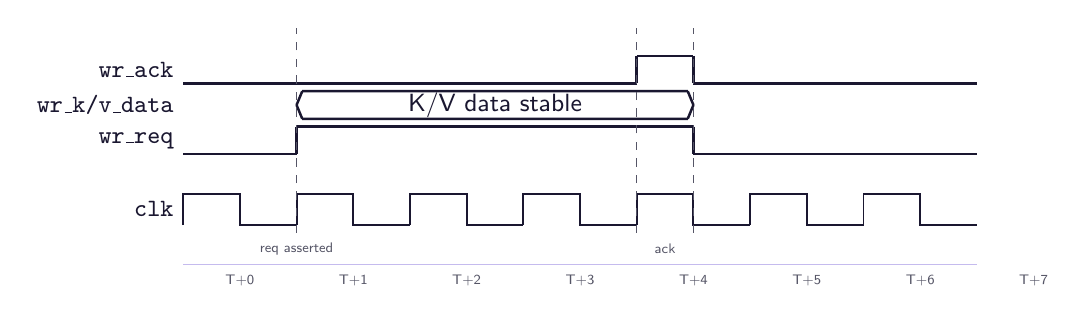
\begin{tikzpicture}[x=0.72cm, y=1cm]
  % Clock
  \foreach \i in {0,2,4,6,8,10,12} {
    \draw[heradark, line width=0.7pt]
      (\i,0) -- (\i,0.4) -- (\i+1,0.4) -- (\i+1,0) -- (\i+2,0);
  }
  \node[left, font=\small, heradark] at (0,0.2) {\portname{clk}};

  % wr_req: goes high at cycle 2, stays until cycle 9
  \wvL{0}{1.25}{2}   \wvR{2}{1.25}   \wvH{2}{1.25}{7}   \wvF{9}{1.25}   \wvL{9}{1.25}{5}
  \node[left, font=\small, heradark] at (0,1.075) {\portname{wr\_req}};

  % wr_k/v_data: valid from cycle 2 to 9
  \wvBus{2}{1.7}{7}{\small K/V data stable}
  \node[left, font=\small, heradark] at (0,1.525) {\portname{wr\_k/v\_data}};

  % wr_ack: one-cycle pulse at cycle 8
  \wvL{0}{2.15}{8}   \wvR{8}{2.15}   \wvH{8}{2.15}{1}   \wvF{9}{2.15}   \wvL{9}{2.15}{5}
  \node[left, font=\small, heradark] at (0,1.975) {\portname{wr\_ack}};

  % Annotations
  \draw[dashed, muted, thin] (2,-0.1) -- (2,2.5);
  \draw[dashed, muted, thin] (8,-0.1) -- (8,2.5);
  \draw[dashed, muted, thin] (9,-0.1) -- (9,2.5);
  \node[font=\tiny, muted] at (2,-0.3) {req asserted};
  \node[font=\tiny, muted] at (8.5,-0.3) {ack};

  % Axis
  \draw[herarule, thin] (0,-0.5) -- (14,-0.5);
  \foreach \i in {0,...,7} {
    \node[font=\tiny, muted] at (\i*2+1,-0.7) {T+\i};
  }
\end{tikzpicture}
\end{center}

\subsection{KV Read Burst}

\portname{rd\_req} is asserted for exactly one cycle with
\portname{rd\_token\_start} and \portname{rd\_token\_end} valid. The engine
asserts \portname{rd\_busy} immediately and streams one beat per cycle on
\portname{rd\_valid}. \portname{rd\_last} is high on the final beat.
Do not assert \portname{rd\_req} while \portname{rd\_busy} is high.

\begin{center}
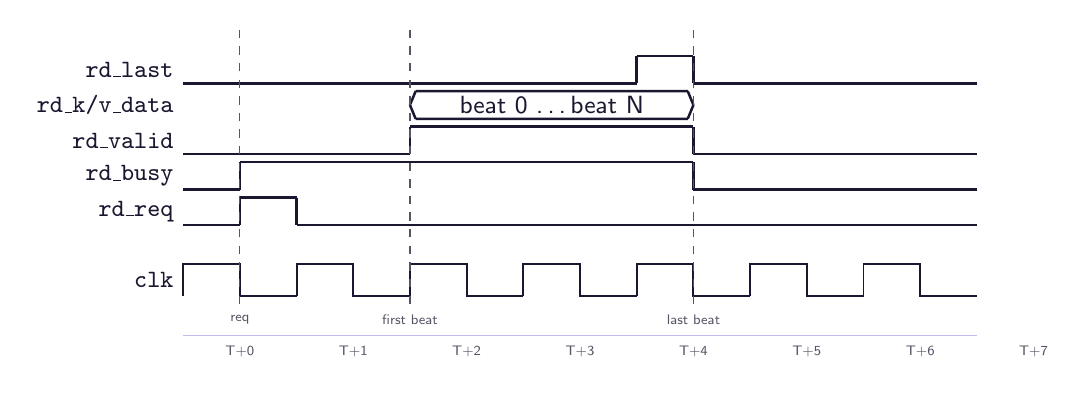
\begin{tikzpicture}[x=0.72cm, y=1cm]
  \foreach \i in {0,2,4,6,8,10,12} {
    \draw[heradark, line width=0.7pt]
      (\i,0) -- (\i,0.4) -- (\i+1,0.4) -- (\i+1,0) -- (\i+2,0);
  }
  \node[left, font=\small, heradark] at (0,0.2) {\portname{clk}};

  % rd_req: one cycle at cycle 1
  \wvL{0}{1.25}{1} \wvR{1}{1.25} \wvH{1}{1.25}{1} \wvF{2}{1.25} \wvL{2}{1.25}{12}
  \node[left, font=\small, heradark] at (0,1.075) {\portname{rd\_req}};

  % rd_busy: high from cycle 1 to cycle 9
  \wvL{0}{1.7}{1} \wvR{1}{1.7} \wvH{1}{1.7}{8} \wvF{9}{1.7} \wvL{9}{1.7}{5}
  \node[left, font=\small, heradark] at (0,1.525) {\portname{rd\_busy}};

  % rd_valid: beats at cycles 4,5,6,7,8
  \wvL{0}{2.15}{4}
  \wvR{4}{2.15} \wvH{4}{2.15}{5} \wvF{9}{2.15}
  \wvL{9}{2.15}{5}
  \node[left, font=\small, heradark] at (0,1.975) {\portname{rd\_valid}};

  % rd_k/v_data: valid beats 4-8
  \wvBus{4}{2.6}{5}{\small beat 0 \ldots beat N}
  \node[left, font=\small, heradark] at (0,2.425) {\portname{rd\_k/v\_data}};

  % rd_last: high on cycle 8
  \wvL{0}{3.05}{8} \wvR{8}{3.05} \wvH{8}{3.05}{1} \wvF{9}{3.05} \wvL{9}{3.05}{5}
  \node[left, font=\small, heradark] at (0,2.875) {\portname{rd\_last}};

  % Annotations
  \draw[dashed, muted, thin] (1,-0.1)  -- (1,3.4);
  \draw[dashed, muted, thin] (4,-0.1)  -- (4,3.4);
  \draw[dashed, muted, thin] (9,-0.1)  -- (9,3.4);
  \node[font=\tiny, muted] at (1,-0.3) {req};
  \node[font=\tiny, muted] at (4,-0.3) {first beat};
  \node[font=\tiny, muted] at (9,-0.3) {last beat};

  \draw[herarule, thin] (0,-0.5) -- (14,-0.5);
  \foreach \i in {0,...,7} {
    \node[font=\tiny, muted] at (\i*2+1,-0.7) {T+\i};
  }
\end{tikzpicture}
\end{center}

\subsection{Soft Reset and Re-initialisation}

After \field{soft\_reset} is pulsed, wait at least 270 clock cycles before
asserting \field{global\_enable} and issuing KV operations. The
\texttt{block\_allocator} requires 256 cycles to repopulate its free list.

\begin{center}
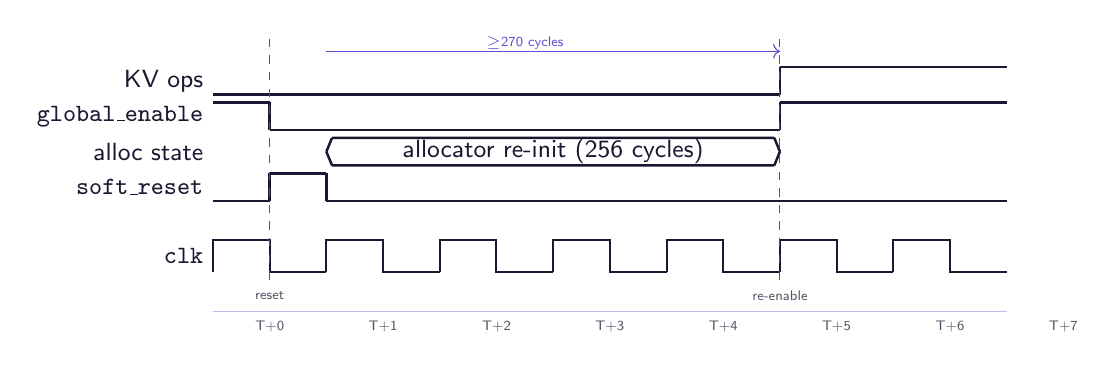
\begin{tikzpicture}[x=0.72cm, y=1cm]
  \foreach \i in {0,2,4,6,8,10,12} {
    \draw[heradark, line width=0.7pt]
      (\i,0) -- (\i,0.4) -- (\i+1,0.4) -- (\i+1,0) -- (\i+2,0);
  }
  \node[left, font=\small, heradark] at (0,0.2) {\portname{clk}};

  % soft_reset pulse at cycle 1
  \wvL{0}{1.25}{1} \wvR{1}{1.25} \wvH{1}{1.25}{1} \wvF{2}{1.25} \wvL{2}{1.25}{12}
  \node[left, font=\small, heradark] at (0,1.075) {\field{soft\_reset}};

  % Allocator init: cycles 2-8 (symbolic; 256 cycles in reality)
  \wvBus{2}{1.7}{8}{\small allocator re-init (256 cycles)}
  \node[left, font=\small, heradark] at (0,1.525) {alloc state};

  % global_enable: goes high at cycle 10
  \wvH{0}{2.15}{1} \wvF{1}{2.15} \wvL{1}{2.15}{9} \wvR{10}{2.15} \wvH{10}{2.15}{4}
  \node[left, font=\small, heradark] at (0,1.975) {\field{global\_enable}};

  % KV ops OK: from cycle 11
  \wvL{0}{2.6}{10} \wvR{10}{2.6} \wvH{10}{2.6}{4}
  \node[left, font=\small, heradark] at (0,2.425) {KV ops};

  \draw[dashed, muted, thin] (1,-0.1)  -- (1,3.0);
  \draw[dashed, muted, thin] (10,-0.1) -- (10,3.0);
  \node[font=\tiny, muted] at (1,-0.3) {reset};
  \node[font=\tiny, muted] at (10,-0.3) {re-enable};
  \node[font=\tiny, muted] at (5.5,2.9)
    {\color{heraviolet}$\geq$270 cycles};
  \draw[heraviolet, ->, thin] (2,2.8) -- (10,2.8);

  \draw[herarule, thin] (0,-0.5) -- (14,-0.5);
  \foreach \i in {0,...,7} {
    \node[font=\tiny, muted] at (\i*2+1,-0.7) {T+\i};
  }
\end{tikzpicture}
\end{center}

% =============================================================================
\section{Synthesis and Performance}
\label{sec:synth}
% =============================================================================

Out-of-context synthesis targeting Artix-7 xc7a100tcsg324-1 (speed grade --1)
at 100\,MHz using Vivado 2018.2. Default parameters:
\param{TOTAL\_PAGES}~=~256, \param{PAGE\_SIZE\_TOKENS}~=~16,
\param{HEAD\_DIM}~=~64, \param{DATA\_WIDTH}~=~16, \param{NUM\_SESSIONS}~=~8.

\subsection{Timing Results}

\renewcommand{\arraystretch}{1.3}
\begin{tabularx}{\linewidth}{L{4cm} L{3cm} X}
\toprule
\textbf{Metric} & \textbf{Value} & \textbf{Notes} \\
\midrule
\rowcolor{tabalt}
Clock period (target) & 10.000\,ns & 100\,MHz \\
WNS (setup)           & +2.079\,ns & 0 failing endpoints \\
\rowcolor{tabalt}
WHS (hold)            & +0.205\,ns & 0 failing endpoints \\
Maximum frequency     & $\approx$126\,MHz & 1\,/\,(10\,--\,2.079)\,ns \\
\rowcolor{tabalt}
Critical path         & 7.921\,ns  & Allocator $\rightarrow$ status decode \\
\bottomrule
\end{tabularx}

\subsection{Resource Utilisation}

\begin{tabularx}{\linewidth}{L{4cm} R{2cm} R{2.5cm} R{2.5cm} R{2.5cm}}
\toprule
\textbf{Resource} & \textbf{Used} & \textbf{Available} & \textbf{Utilisation} & \textbf{xc7a35t equiv.} \\
\midrule
\rowcolor{tabalt}
Slice LUTs      & 10,191 & 63,400  & 16.07\,\% & 49.0\,\% \\
Slice Registers & 12,533 & 126,800 & \phantom{0}9.88\,\% & 30.1\,\% \\
\rowcolor{tabalt}
Block RAM Tiles &    116 &    135  & 85.93\,\% & $>$\,100\,\% \\
DSPs            &      0 &    240  & \phantom{00}0.00\,\% & 0.0\,\% \\
\bottomrule
\end{tabularx}

The synthesis script is provided at \texttt{synth\_hera.tcl} in the repository
root for full reproducibility.

\subsection{BRAM Scaling}

\notebox[Integration note]{At full parameters, Hera consumes 116 of 135 BRAM
tiles on the xc7a100t ($\approx$86\,\%), leaving minimal headroom for
surrounding logic. Reduce \param{TOTAL\_PAGES} or \param{HEAD\_DIM} for
Artix-7 integration, or target a device with greater BRAM capacity.
BRAM and LUTRAM usage scale linearly with
$\param{TOTAL\_PAGES} \times \param{HEAD\_DIM}$.}

\renewcommand{\arraystretch}{1.3}
\begin{tabularx}{\linewidth}{C{2.5cm} C{2.2cm} C{2.6cm} C{2.4cm} C{3.5cm}}
\toprule
\param{TOTAL\_PAGES} & \param{HEAD\_DIM} & SRAM footprint & BRAM tiles (est.) & xc7a100t utilisation \\
\midrule
\rowcolor{tabalt} 64  & 32 & 128\,KB & $\approx$29  & $\approx$21\,\% \\
                 128  & 64 & 512\,KB & $\approx$58  & $\approx$43\,\% \\
\rowcolor{tabalt} 256 & 64 &   1\,MB &         116  &         85.9\,\% \\
                  512 & 64 &   2\,MB & $\approx$232 & $>$100\,\% — use UltraScale+ \\
\rowcolor{tabalt} 256 & 128&   2\,MB & $\approx$232 & $>$100\,\% — use UltraScale+ \\
\bottomrule
\end{tabularx}

% =============================================================================
\section{Integration Guidelines}
% =============================================================================

\subsection{Initialisation Sequence}

\begin{enumerate}
  \item Assert \portname{rst\_n} low for $\geq$2 clock cycles (hard reset).
  \item Configure \reg{SESSION\_CFG}, \reg{PAGE\_CFG}, and \reg{IRQ\_MASK}
        as required for the application.
  \item Optionally write \reg{LOCK[0]}~=~1 to freeze configuration.
  \item Write \reg{CTRL[0]}~=~1 (\field{global\_enable}).
  \item Wait $\geq$270 clock cycles for the \texttt{block\_allocator}
        to complete its free-list initialisation pass.
  \item Begin issuing KV write and read operations.
\end{enumerate}

After a soft reset (\reg{CTRL[1]} pulse), repeat steps 4–6.
\reg{LOCK} state is preserved across a soft reset.

\subsection{AXI4-Lite Interconnect Requirements}

\begin{itemize}
  \item Address width: 32 bits (bits [31:8] are ignored; only [7:0] are decoded).
  \item Data width: 32 bits; byte strobes are accepted but sub-word writes are
        not recommended.
  \item Write-address and write-data channels may arrive in the same cycle.
  \item Outstanding transactions: the slave accepts one outstanding write and
        one outstanding read at a time. Use a 1-deep FIFO or tie off if the
        interconnect requires bursts or ordering.
  \item There are no memory-type or cache attributes — connect
        \portname{s\_axi\_arprot} and \portname{s\_axi\_awprot} to \hex{000}
        or leave undriven.
\end{itemize}

\subsection{Security Considerations}

\begin{itemize}
  \item Assign each session to a single AI inference context or tenant.
        The hardware enforces isolation, but the session ID must be set by
        trusted firmware before submitting KV operations.
  \item Set \reg{PAGE\_CFG.max\_pages\_per\_session} to a non-zero value
        to prevent a single session from exhausting the page pool.
  \item Write \reg{LOCK[0]}~=~1 after boot-time configuration to prevent
        runtime reconfiguration of session boundaries and quotas.
  \item Monitor \portname{irq} and \reg{STATUS.sec\_fault}. A latched
        \field{sec\_fault} indicates an attempted cross-session access
        and should be treated as a security event.
\end{itemize}

\subsection{Clocking and Reset}

\begin{itemize}
  \item Hera is a single-clock design. All ports must be driven from the
        same clock domain as \portname{clk}.
  \item \portname{rst\_n} is asynchronous and active-low. It is safe to
        release it synchronously on the rising edge.
  \item A minimum de-assertion pulse of 2 clock cycles is required to
        guarantee all reset registers have settled before operation resumes.
\end{itemize}

% =============================================================================
\section{Verification}
% =============================================================================

The testbench (\texttt{sim/tb\_sv\_top.sv}) is a zero-UVM class-based
SystemVerilog testbench that runs on Vivado xsim 2018.2 without
additional dependencies.

\renewcommand{\arraystretch}{1.3}
\begin{tabularx}{\linewidth}{L{4.5cm} C{2cm} C{2.5cm} X}
\toprule
\textbf{Test} & \textbf{Checks} & \textbf{Result} & \textbf{Coverage} \\
\midrule
\rowcolor{tabalt}
Smoke — reset, enable, single write/read &
  14 & \textbf{\color{green!50!black}PASS} &
  Basic data path, AXI transactions, watermark \\
Stress — 128 writes across 8 sessions, 16 scoreboard reads &
  11 & \textbf{\color{green!50!black}PASS} &
  All sessions exercised, quota enforcement \\
\rowcolor{tabalt}
Security — isolation, quota, LOCK, SLVERR &
  10 & \textbf{\color{green!50!black}PASS} &
  Cross-session rejection, LOCK stickiness, watermark \\
Soft Reset — zero-on-free, re-init, re-write &
  6  & \textbf{\color{green!50!black}PASS} &
  Reset sequencing, scrub verification \\
\midrule
\textbf{Total} & \textbf{41} & \textbf{\color{green!50!black}PASS} & \\
\bottomrule
\end{tabularx}

\vspace{4pt}

Run the testbench with:
\begin{center}
\texttt{cd sim \&\& run\_xsim.bat}
\end{center}

% =============================================================================
\section{Parameters}
% =============================================================================

\renewcommand{\arraystretch}{1.3}
\begin{tabularx}{\linewidth}{L{4.2cm} C{2cm} C{2cm} X}
\toprule
\textbf{Parameter} & \textbf{Default} & \textbf{Range} & \textbf{Description} \\
\midrule
\rowcolor{tabalt}
\param{TOTAL\_PAGES}      & 256 & 1–256  &
  Number of physical SRAM pages. Directly scales BRAM and LUTRAM usage. \\
\param{PAGE\_SIZE\_TOKENS}& 16  & 1–64   &
  Tokens per page. Together with \param{TOTAL\_PAGES}, determines the total
  token capacity. \\
\rowcolor{tabalt}
\param{HEAD\_DIM}         & 64  & 1–128  &
  Attention head dimension (number of elements per KV vector).
  Scales BRAM linearly. \\
\param{NUM\_SESSIONS}     & 8   & 1–8    &
  Number of concurrent sessions. Fixed at 3-bit encoding; maximum is 8. \\
\rowcolor{tabalt}
\param{DATA\_WIDTH}       & 16  & 8, 16  &
  Bit width of each KV element. 16 = FP16. \\
\param{SRAM\_BANKS}       & 4   & 4      &
  Number of interleaved SRAM banks. Fixed at 4; do not modify. \\
\bottomrule
\end{tabularx}

% =============================================================================
\section{Revision History}
% =============================================================================

\renewcommand{\arraystretch}{1.3}
\begin{tabularx}{\linewidth}{C{1.4cm} C{2.2cm} L{3.5cm} X}
\toprule
\textbf{Version} & \textbf{Date} & \textbf{Author} & \textbf{Description} \\
\midrule
\rowcolor{tabalt}
1.0 & June 2026 & Circle &
  Initial public release. Full feature set: paged allocation, scatter-gather
  read/write, LRU eviction, sequential prefetch, multi-tenant isolation,
  AXI4-Lite control interface. Synthesised on Artix-7 xc7a100t at 100\,MHz;
  41/41 simulation checks passing. \\
\bottomrule
\end{tabularx}

\vspace{6mm}
\noindent{\color{herarule}\rule{\linewidth}{0.5pt}}

\vspace{4pt}
\begin{center}
  \small\color{muted}
  Copyright \textcopyright{} 2026 Circle.
  Licensed under the Apache License, Version 2.0.\\[2pt]
  \href{https://github.com/anubhavgpta/hera}{github.com/anubhavgpta/hera}
  \enspace\textbullet\enspace
  \href{mailto:anubhavgpta@outlook.com}{anubhavgpta@outlook.com}
\end{center}

\end{document}
